
\documentclass{beamer} 


\mode<presentation>
{
  \usetheme{Berkeley}
  % or ...

  \setbeamercovered{transparent}
  % or whatever (possibly just delete it)
}

\usepackage{tikz}
\usepackage{graphicx}
\usepackage[english]{babel}
% or whatever

\usepackage[utf8]{inputenc}
% or whatever

\usepackage{times}
\usepackage[T1]{fontenc}
% Or whatever. Note that the encoding and the font should match. If T1
% does not look nice, try deleting the line with the fontenc.


\title[] % (optional, use only with long paper titles)
{Tools for a Reproducible Workflow}

\subtitle
{}

\author[Christensen] % (optional, use only with lots of authors)
{Garret~Christensen\inst{1}}
% - Give the names in the same order as the appear in the paper.
% - Use the \inst{?} command only if the authors have different
%   affiliation.

\institute[Universities of Somewhere and Elsewhere] % (optional, but mostly needed)
{
  \inst{1}%
  UC Berkeley:\\
  Berkeley Initiative for Transparency in the Social Sciences\\
  Berkeley Institute for Data Science\\
  }
% - Use the \inst command only if there are several affiliations.
% - Keep it simple, no one is interested in your street address.

\date[BITSS2014] % (optional, should be abbreviation of conference name)
{IMEBESS, April 2017\\
Slides available online at \url{https://github.com/BITSS/UCMerced2017}}
% - Either use conference name or its abbreviation.
% - Not really informative to the audience, more for people (including
%   yourself) who are reading the slides online

\subject{Research Transparency}
% This is only inserted into the PDF information catalog. Can be left
% out. 

\pgfdeclareimage[height=2cm]{university-logo}{../Images/BITSSlogo.png}
\logo{\pgfuseimage{university-logo}}

% If you have a file called "university-logo-filename.xxx", where xxx
% is a graphic format that can be processed by latex or pdflatex,
% resp., then you can add a logo as follows:

% \pgfdeclareimage[height=0.5cm]{university-logo}{university-logo-filename}
% \logo{\pgfuseimage{university-logo}}



% Delete this, if you do not want the table of contents to pop up at
% the beginning of each subsection:
%\AtBeginSubsection[]
%{
%  \begin{frame}<beamer>{Outline}
%    \tableofcontents[currentsection,currentsubsection]
%  \end{frame}
%}


% If you wish to uncover everything in a step-wise fashion, uncomment
% the following command: 

\beamerdefaultoverlayspecification{<+->}


\begin{document}

\begin{frame}
  \titlepage
\end{frame}




% Structuring a talk is a difficult task and the following structure
% may not be suitable. Here are some rules that apply for this
% solution: 

% - Exactly two or three sections (other than the summary).
% - At *most* three subsections per section.
% - Talk about 30s to 2min per frame. So there should be between about
%   15 and 30 frames, all told.

% - A conference audience is likely to know very little of what you
%   are going to talk about. So *simplify*!
% - In a 20min talk, getting the main ideas across is hard
%   enough. Leave out details, even if it means being less precise than
%   you think necessary.
% - If you omit details that are vital to the proof/implementation,
%   just say so once. Everybody will be happy with that.
%%%%%%%%%%%%%%%%%%%%%%%%%%%%%%%%%%%%%%%%%%%%%%%%%%%%%%%%%%%%%%%%%%%%%%%
%%%%%%%%%%%%%%%%%%%%%%%%%%%%%%%%%%%%%%%%%%%%%%%%%%%%%%%%%%%%%%%%%%%%%

\section {Introduction}
{ % all template changes are local to this group.
    \setbeamertemplate{navigation symbols}{}
    \begin{frame}[plain]
        \begin{tikzpicture}[remember picture,overlay]
            \node[at=(current page.center)] {
                \href{https://www.bitss.org/}{\includegraphics[width=\paperwidth]{../Images/bitsslogo.png}}
            };
        \end{tikzpicture}
     \end{frame}
}


%%%%%%%%%%%%%%%%%%%%%%%%%%%%%%%%%%%%%%%%%%%%%%%%%%%%%%%%%%%%%%%%%%%%%%%%%%%

 \section{Workflow}
 \begin{frame}{Workflow}
``Reproducibility is just collaboration with people you don't know,
including yourself next week''

---Philip Stark, UC Berkeley Statistics
\end{frame}
\begin{frame}{Workflow}

 \begin{itemize}[<.->]
 \item OSF
 \item Version Control
 \item Dynamic Documents
\end{itemize}
\end{frame}

\begin{frame}
Put your work all in one place with the Open Science Framework \href{http://osf.io}{\beamerbutton{Link}}
\begin{itemize}[<.->]
\item Pre-Registration
\item Data
	\begin{itemize}
	\item Host
	\item Link to Dataverse
	\end{itemize}
\item Version Control
\item More to Come
\end{itemize}
\end{frame}

{
% all template changes are local to this group.
    \setbeamertemplate{navigation symbols}{}
    \begin{frame}[plain]
         \begin{tikzpicture}[remember picture,overlay]
            \node[at=(current page.center)] {
                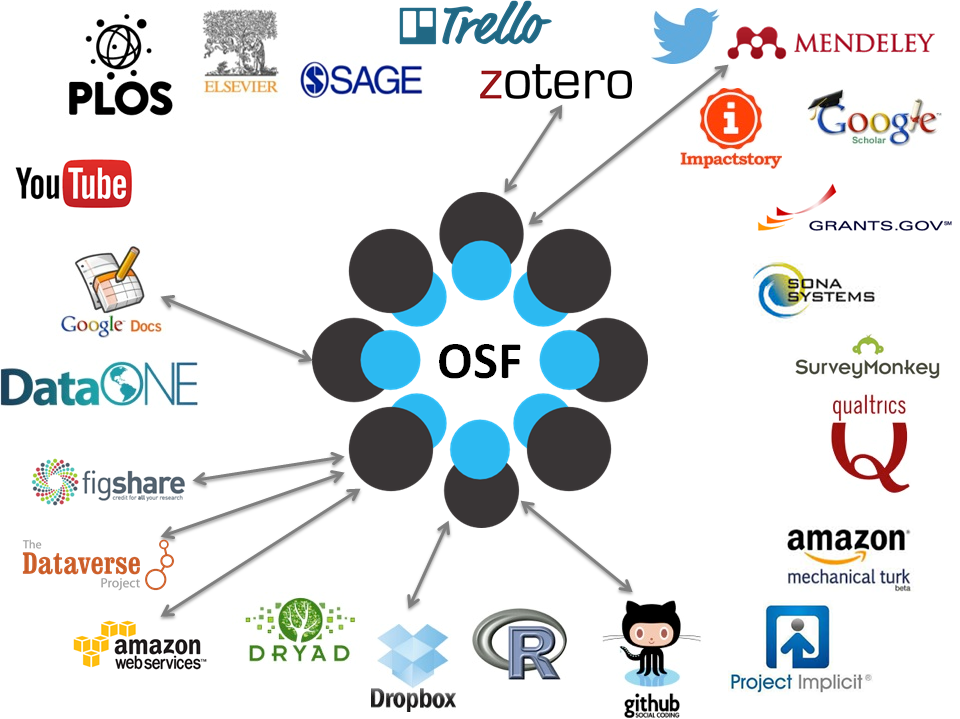
\includegraphics[width=\paperwidth]{../Images/OSFnow.PNG}
            };
        \end{tikzpicture}
     \end{frame}

% all template changes are local to this group.
    \setbeamertemplate{navigation symbols}{}
    \begin{frame}[plain]
         \begin{tikzpicture}[remember picture,overlay]
            \node[at=(current page.center)] {
                
\includegraphics[width=\paperwidth]{../Images/OSFsoon.PNG}
            };
        \end{tikzpicture}
     \end{frame}

 % all template changes are local to this group.
    \setbeamertemplate{navigation symbols}{}
    \begin{frame}[plain, label=AEAreg]
         \begin{tikzpicture}[remember picture,overlay]
            \node[at=(current page.center)] {
                
\includegraphics[height=\paperheight]{../Images/github-logo-transparent.JPG}
            };
        \end{tikzpicture}
     \end{frame}
}


\begin{frame}{Dynamic Documents}
Write your code and your paper in the same file so you won't lose information or make copy and paste mistakes.

\begin{itemize}[<.->]
\item Include tables by linking to a file, instead of a static image.
\item Include number by linking to a value calculated by an analysis file, instead of a static number typed manually.
\item Automatically update tables and numbers.
\item Produce entire paper with one or two clicks.
\end{itemize} 
\end{frame}

\begin{frame}{Dynamic Documents}
Possible in Python, R, and to a lesser extent, Stata

\begin{itemize}[<.->]
\item Jupyter---several (many?) languages
\item R---use R Studio to manage projects with built-in version control, and R Markdown/knitr for publication-quality dynamic documents.
\item Stata--combine with LaTeX for two click workflow
\item Stata--use `\href{https://github.com/haghish/MarkDoc}{markdoc}' ado for some dynamic ability.
\end{itemize} 
\end{frame}

 
 { % all template changes are local to this group.
    \setbeamertemplate{navigation symbols}{}
    \begin{frame}[plain, label=AEAreg]
         \begin{tikzpicture}[remember picture,overlay]
            \node[at=(current page.center)] {
                
\includegraphics[width=\paperwidth]{../Images/RStudio-Logo-Blue-Gradient.png}
            };
        \end{tikzpicture}
     \end{frame}
}

{ % all template changes are local to this group.
    \setbeamertemplate{navigation symbols}{}
    \begin{frame}[plain, label=AEAreg]
         \begin{tikzpicture}[remember picture,overlay]
            \node[at=(current page.center)] {
                
\includegraphics[height=\paperheight]{../Images/jupyter.png}
            };
        \end{tikzpicture}
     \end{frame}
}

\section{Conclusion}
\begin{frame}{Conclusion}
OK, I'm convinced. How do I learn more?

\begin{itemize}[<.->]
\item Work through my demos.\href{https://github.com/BITSS/UCMerced2017}{\beamergotobutton{Link}}
\item Software Carpentry's tutorials \href{http://www.software-carpentry.org/lessons}{\beamergotobutton{Link}}

\end{itemize}
\end{frame}


\end{document}

